
% this file is called up by thesis.tex
% content in this file will be fed into the main document

%: ----------------------- introduction file header -----------------------


\begin{savequote}[50mm]
I am not young enough to know \mbox{everything}.
\qauthor{Oscar Wilde}
% The beginning is the most important part of the work.
% \qauthor{Plato}
\end{savequote}

%\chapter{Localization methods, techniques and technologies}
\chapter{Localization Background}
\label{cha:2_positioning}

% the code below specifies where the figures are stored
\ifpdf
    \graphicspath{{2_positioning/figures/PNG/}{2_positioning/figures/PDF/}{2_positioning/figures/EPS/}}
\else
    \graphicspath{{2_positioning/figures/EPS/}{2_positioning/figures/}}
\fi

The aim of this chapter is to provide an overview of the problem of localization, presenting the main methods, techniques and technologies that exist in the state of the art for its resolution.
In this way, it is intended to reinforce the motivation introduced in the previous chapter on the importance of methods based on inertial sensor in achieving seamless positioning solutions for pedestrians.
Therefore, a reader with experience in the field of localization systems may choose to skip this chapter.

Section~\ref{sec:2_1_intro} presents a brief historical overview of navigation and localization systems and defines several basic concepts.
Then, Section~\ref{sec:2_2_positionFix} and Section~\ref{sec:2_3_DR} describe the two main localization methods: position fixing and DR.
Later, Section~\ref{sec:2_4_fusion} provides a brief description about the benefits of information fusion and the most common techniques applied for localization.
Section~\ref{sec:2_5_AHRS} introduces the Attitude and Heading Reference Systems, a concept closely related to localization systems based on DR that is frequently used.
Finally, Section~\ref{sec:2_6_summary} summarizes the contents and main conclusions of this chapter.
\section{Introduction}
\label{sec:2_1_intro}
Since the beginning of time, human beings have had different reasons to move and travel, either to find new sources of food, places with a milder climate or better conditions, or because of the mere desire to explore, driven by their innate curiosity.
Subsequently, the expansion of trade and the inevitable wars created the need to record, plan and conduct such journeys in a more efficient and secure manner, as larger distances were being covered. 
Therefore, the science and art of navigation has been the main application and motivation that has led to the search and design of increasingly more accurate and advanced localization systems, methods and techniques.

Numerous advances have been made in this area throughout history, the following being some of the most notable:
% \cite{grewal_global_2001, titterton_strapdown_2004, bowditch_originally_by_american_2017, walter_history_2007, prieto_tejedor_estimacion_2012, zampella_localizacion_2017}:
\begin{itemize}	
	\item Celestial Navigation: When traveling on land or in ships close to the shore, the observation of known landmarks allows the navigation. This technique is called piloting or pilotage \cite{bowditch_originally_by_american_2017}. However, this is more difficult when traveling around unknown areas or where there are no clear landmarks, such as when moving away from the coast. For more than two thousand years, people like the Polynesians or the Phoenicians began to use the different celestial bodies as a references \cite{titterton_strapdown_2004}. The latter used Polaris (now Polar Star) as a reference for the northern direction, as its position in the sky is so close to the Earth's axis of rotation that it appears static every night.
	\item Compass: The use of the celestial bodies as a reference is subject to clear skies. There is evidence that the Vikings and the Chinese discovered the properties of magnetite more than a thousand years ago, which allowed them to navigate even in situations where the sky was not visible \cite{titterton_strapdown_2004}. This discovery allowed the development of the DR technique, by means of which it is possible to obtain the trajectory by updating a known initial position using the measured speeds and orientations \cite{bowditch_originally_by_american_2017}.
	\item Sextant and chronometer: The use of astrolabes and then sextants made it possible to measure latitude by observing the elevation of different stars, usually the sun, relative to the horizon. However, calculation of the longitude was a problem for a longer period of time, as it required high precision clocks to know the time in a given reference meridian. It was not until 1761 that John Harrison managed to design a chronometer with an error of 1 second a day, which allowed to determine the longitude with an acceptable error~\cite{titterton_strapdown_2004}.
	\item Radio Navigation: Since the end of the 19th century, the contributions of figures such as Maxwell, Hertz and Marconi, among others, established the electromagnetic theory and the use of radio communications. During the World War II, considerable progress was made in this area, and from that moment on, localization systems based on electromagnetic waves began to emerge. From the first hyperbolic systems such as the Gee, the LORAN, the Omega or the Decca to the current GNSS such as the American GPS (1973), the Russian GLONASS (1976) or the European Galileo (2003) \cite{groves_principles_2008}.
	\item Inertial Navigation: In the early 20th century, the first ideas emerged about the possibility of designing a self-contained navigation device that would be capable of tracking the trajectory of an object by detecting changes in its inertia, as indicated by the theory of mechanics established by Isaac Newton three centuries earlier \cite{bray_you_2014}.
	Once again, with the advances made during the World War II in the technology of inertial sensors for use mainly in missile guidance, it was possible to build the first really useful INS systems, and their use was quickly extended to the navigation of any means of transport. Since the end of the 20th century, and thanks to MEMS technology, it has been possible to manufacture inertial sensors of low cost, size and weight, which allows them to be installed in many portable devices, such as smartphones, and to be used for a wide variety of applications \cite{grewal_global_2001,titterton_strapdown_2004, walter_history_2007}.
\end{itemize}
		
% As can be seen, the major advances in localization have mainly come from the field of navigation, whose application scenarios are usually large, open and generally undisturbed places.
% However, as noted in Chapter~\ref{cha:1_Introduction}, the new paradigms of ubiquitous computing, context-aware system and LBS can not be restricted only to such scenarios since they require seamless localization information, including in highly complex scenarios. 
As can be seen, great advances in the field of localization have come mainly from applications whose cases of use take place mostly in large outdoor spaces.
However, as noted in Chapter~\ref{cha:1_Introduction}, the new paradigms of ubiquitous computing require location information in a seamless way and in any type of scenario.
In addition, the desire to provide such a seamless localization to pedestrians on a massive scale implies the use of portable and inexpensive devices, which imposes additional restrictions and requirements that motivate the need to search for new localization methods. 
A good review of the main requirements that can be asked of a localization system can be found in the work of Rainer Mautz \cite{mautz_rainer_indoor_2012}, which he summarized in the Figure~\ref{fig:IPS_req_mautz}.

%\InsertFig{IPS_req_mautz.png}{fig:IPS_req_mautz}{User requirements for a localization system}{Source: Rainer Mautz \cite{mautz_rainer_indoor_2012}}{1}{}
% \InsertFig{Mautz_reqs_vectorial_text}{fig:IPS_req_mautz}{User requirements for a localization system}{Source: Rainer Mautz \cite{mautz_rainer_indoor_2012}}{1}{}
\begin{figure}[!t]
    \centering
	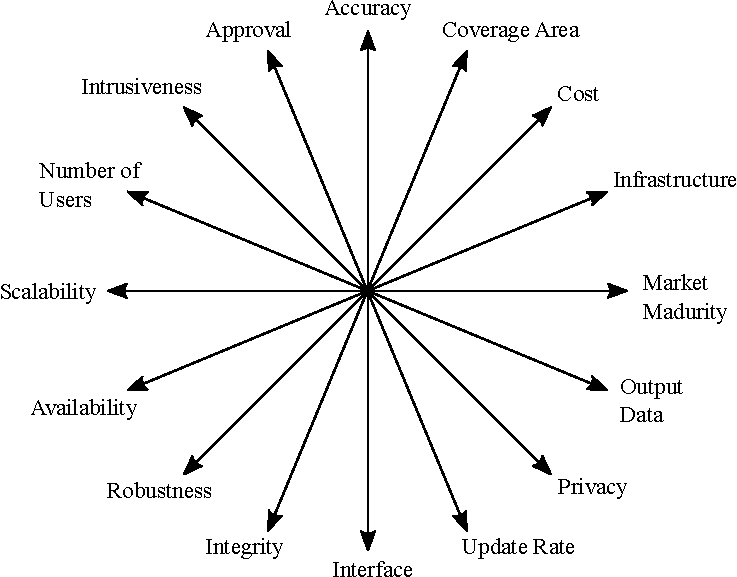
\includegraphics[width=\textwidth]{Mautz_reqs_vectorial_text}    	
	\caption[User requirements for a localization system]{User requirements for a localization system. Source: Rainer Mautz \cite{mautz_rainer_indoor_2012}.}
	\label{fig:IPS_req_mautz}
\end{figure}

Before going on, it is convenient to clarify a series of concepts and terms that, although often used as synonyms, have different nuances:
\begin{itemize}
	\item Localization and Position: In English, to localize and to position are often used interchangeably, but there is a slight nuance. In general, it can be thought that localization is a more abstract concept, which determines the spatial relations between objects. In this way, the localization can be symbolic (I am at home), or physical (latitude and longitude). Therefore, the position could be seen as a type of physical localization, such as the coordinates in a reference system. Thus, all positioning systems are localization systems, but not necessarily the other way around.	
	\item Navigation: This term includes any method of determining and planning the trajectory of an object. Therefore, it requires knowledge of its position, velocity and orientation with respect to a reference frame. Consequently, all navigation systems should include a positioning system and, depending on how the localization information is computed and provided, localization systems can also be navigation systems. For this reason, both terms are sometimes used as synonyms.
	\item Tracking: It differs from navigation in that the position and speed is obtained by an external agent, without necessarily requiring the installation of equipment on the object being tracked.	
\end{itemize}

As can be deduced from the list of historical milestones seen above, there are five main navigation/localization techniques: pilotage, celestial navigation, DR, radio navigation and inertial navigation \cite{grewal_global_2001}. 
However, all of them can be categorized in two main general localization methods:
on the one hand, the so-called position fixing methods, in which the element that calculates the localization uses information received or collected from the environment; and, on the other hand, DR-based methods, in which the element interested in its position is able to calculate it autonomously from changes in its inertia, updating known initial position and orientation.
The following Sections~\ref{sec:2_2_positionFix} and \ref{sec:2_3_DR} will review the general concepts of each of these two localization methods, as well as the main techniques and technologies used to implement them.